\section{Results}
Figure~\ref{fig:inf.toroth} illustrates modelled \MPXV incidence and cumulative infections
in city~A versus city~B under different strategies for vaccine allocation.
Because of the larger population size,
greater epidemic potential ($R_0$), and
having all imported/seed cases in city~A in this scenario,
allocating all 5000 vaccine doses to city~A
yielded the fewest infections (550; solid line) by day~90 (optimal strategy). % MAN
Allocating vaccines proportionally to city size yielded 615 infections (broken line),
whereas no vaccination yielded 1020 infections (dotted line)
(Figure~\ref{fig:inf.toroth}\,I; corresponding incidence rates in Figure~\ref{fig:inf.toroth}\,J).
\par
Allocating most/all doses to city~A
allowed incidence to rise exponentially in city~B.
However, this approach can still avert more infections overall over shorter time horizons,
after which more doses may become available.
Figure~\ref{fig:inf.base} illustrates the opposite case
(default model parameters in Table~\ref{tab:model.params}): two identical cities with equal seeding,
where the optimal allocation is equal between cities.
\begin{figure}[h]
  \centerline{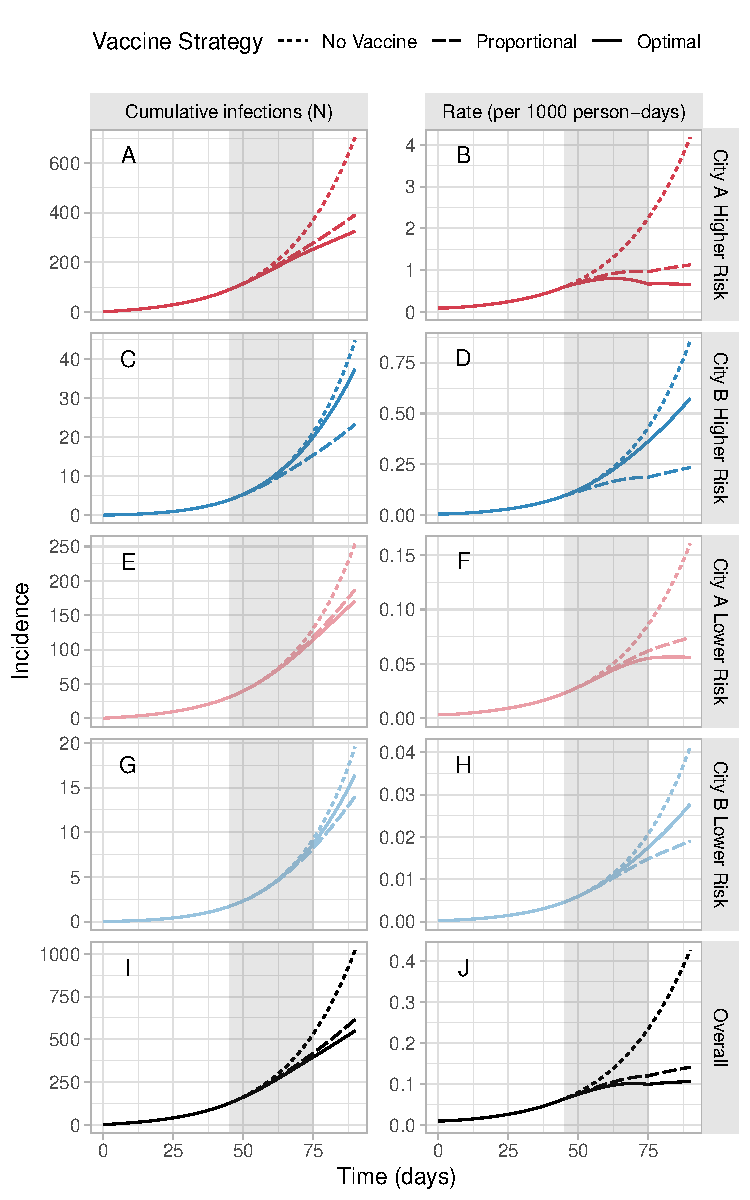
\includegraphics[width=.8\textwidth]{inf.toroth}}
  \caption{Modelled \MPXV cumulative infections and incidence in two cities
    under three different vaccine allocation scenarios}
  \label{fig:inf.toroth}
  \floatfoot
  Gray bar indicates period of vaccine roll-out (days 45--75).
  City~A reflects a Toronto-like city and city~B reflects a medium-sized city in Ontario.
  For vaccine allocation,
  proportional allocation (to city size) was 75\% to city~A and 25\% to city~B; while
  optimal allocation (most infections averted by day~90) was 100\% to city~A.
  Risk: risk of \MPXV infection or transmission, defined by
  numbers of sexual partners (definitions in Appendix~\ref{app.model}.)
\end{figure}
\par
Figure~\ref{fig:grid.opt} illustrates optimal vaccine allocation between cities A~and~B
across different epidemic conditions.
Figures~\ref{fig:grid.dci.none}--\ref{fig:grid.rdci.prop} further illustrate the
absolute and relative numbers of infections averted under optimal allocation
versus no vaccination (\ref{fig:grid.dci.none}--\ref{fig:grid.rdci.none}), and
versus vaccine allocation proportional to city size (\ref{fig:grid.dci.prop}--\ref{fig:grid.rdci.prop}),
showing under what conditions optimal allocation is most important.
\par
We found that the strongest determinants of optimal vaccine allocation were:
relative epidemic potential ($R_0$), share of seed cases, and city size,
although the size of the higher-risk group was proportional to
city size under our modelling assumptions.
Thus, if a larger city had a large $R_0$ and most of the seed cases,
it was best to allocate most/all doses to that city in our analysis
(solid red/blue corners in Figure~\ref{fig:grid.opt}).
\par
% TODO: higher/lower risk
For smaller cities with large $R_0$ and most of the seed cases,
it was sometimes possible to vaccinate the entire higher risk group;
in such instances, the remaining doses were best allocated to
the higher risk group in the other city,
yielding the plateaus (solid yellow triangles) in Figure~\ref{fig:grid.opt}:
(A,D,G) upper right; (C,F,I) lower left.
This plateau shows how priority populations can change
if/after high levels of coverage are achieved in other populations.
\par
When cities with most/all seed cases had smaller $R_0$,
doses were shared between cities under the optimal allocation strategy (to varying degrees),
which suggests that both risk-based (reflecting $R_0$) and
proximity-based (reflecting initial cases) prioritization strategies
worked together to minimize transmission.
In such instances, the other city necessarily had few/no seed cases but larger $R_0$,
to which the same findings apply.
These conditions are represented by the yellow diagonal segments
in all facets of Figure~\ref{fig:grid.opt}.
\par
Increased levels of mixing between cities
mainly acted to reduce the influence of initial seed cases,
and increase the influence of $R_0$
on optimal allocation of vaccines to each city (shown by the
stronger vertical gradients [contours are relatively more horizontal]
in Figure~\ref{fig:grid.opt} [A,B,C] with more inter-city mixing, versus
stronger horizontal gradients [contours are relatively more vertical]
in [G,H,I] with less inter-city mixing).
\begin{figure}
  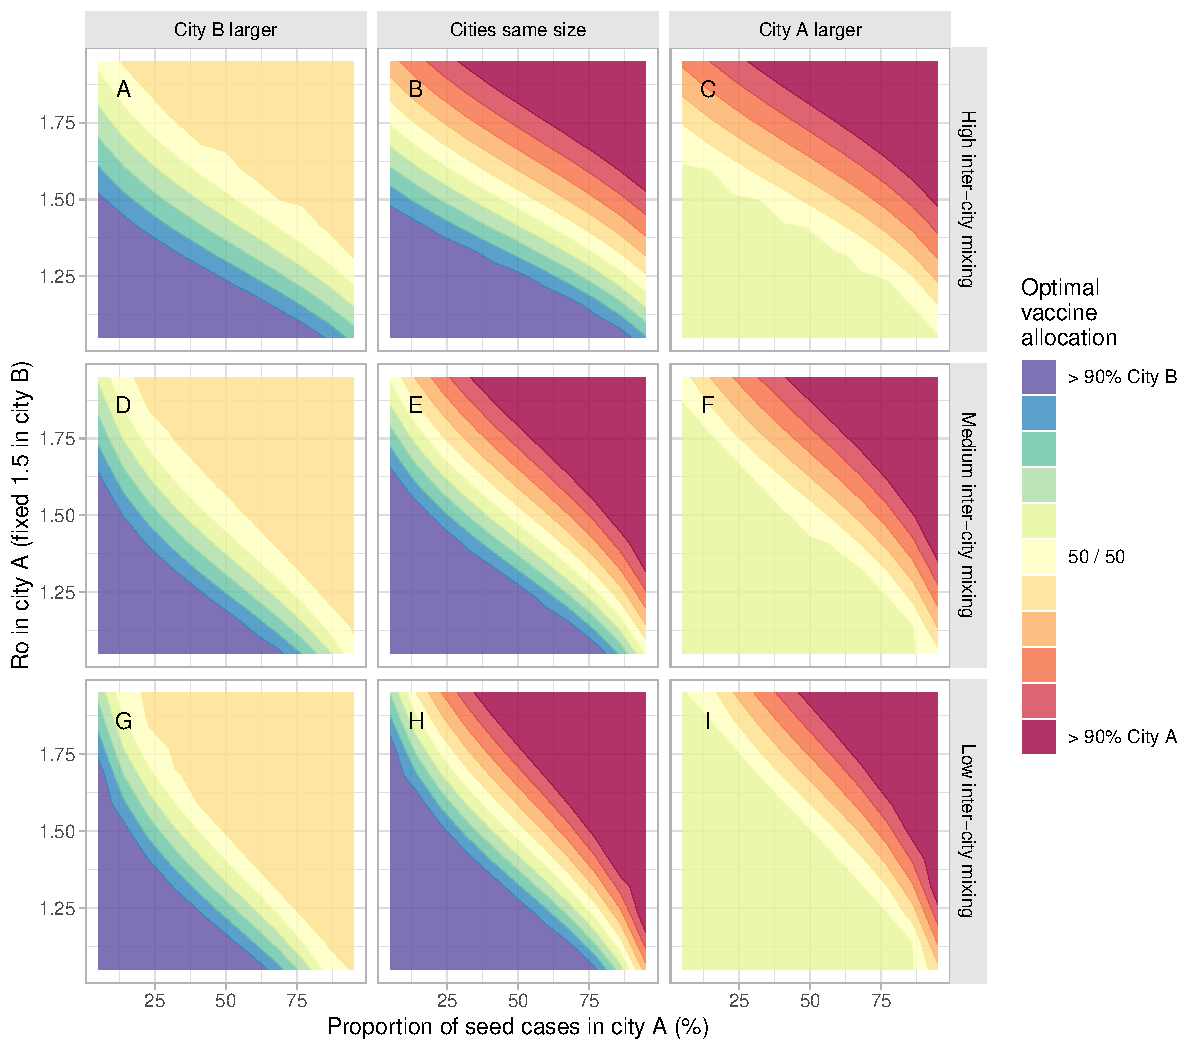
\includegraphics[width=\linewidth]{grid.opt.pdf}
  \caption{Optimal \MPXV vaccine allocation between two cities
    under different epidemic conditions}
  \label{fig:grid.opt}
  \floatfoot
  \gridfoot
\end{figure}
